\chapter{Une solution orientée BDD}
\label{chap:secondchapitre}

\section{Un DSL pour modéliser les exigences}

Nous avons montré dans la première partie la pertinence de la modélisation des exigences pour générer des tests fonctionnels. La modélisation qui répond au mieux à nos critères sont les DSL.  Nous avons vu que des outils comme Cucumber permettent à partir du DSL Gherkin ou encore EasyB, de passer des exigences à des tests.  Dans ces outils le DSL mis en place représente un scénario qui décrit un comportement du logiciel. Il s’agit donc d’une approche Behaviour Driven Developpement. Dans la solution que nous proposons, nous souhaitons garder ces éléments que nous pensons pertinents. Par conséquent, les personnes en charge de la rédaction des exigences devront se conformer au formalisme imposé par le DSL pour rédiger les exigences. Etant donné que le DSL représente un scénario qui est une modélisation connue des rédacteurs d'exigences et qui est une modélisation proche du langage naturel, nous pensons qu'il sera simple pour toutes les parties prenantes de lire et d'écrire les exigences dans ce format. 
Dans l'exemple que nous allons dérouler nous décidons de prendre comme DSL Gherkin et le langage Java pour l'implantation des méthodes mais la logique que nous proposons est tout à fait applicable à d'autres langages de programmation. Toutefois, il est possible qu'une entreprise souhaite développer son propre DSL car les spécificités de son domaine n'existent dans aucun DSL déjà programmé. Le nouveau DSL  devra imposer une structure qui permettra de déterminer quels sont les mots clés à partir desquels il faut générer une méthode de test. Dans le cas de Gherkin les termes "Scenario", "When", "And", "Given", "Then" du DSL permettent de générer une méthode de test à implanter. 

            \begin{figure}[H]
                \centering
                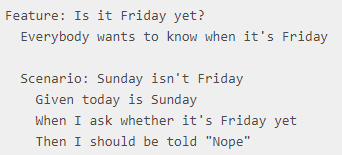
\includegraphics[width=\textwidth]{images/dsldsl.PNG}
                \caption{Exemple de scénario avec un DSL Gherkin}
            \end{figure}

\section{Génération des méthodes de test}

Une fois les exigences rédigées dans le DSL, pour chaque mot clé une signature de méthode est générée. Par exemple avec Cucumber : 

            \begin{figure}[H]
                \centering
                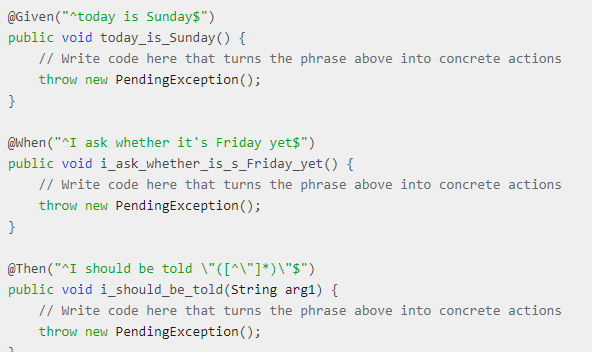
\includegraphics[width=\textwidth]{images/fixture.PNG}
                \caption{Exemple de méthodes de tests générés avec Cucumber}
            \end{figure}

Dans le corps de chaque méthode générée, un commentaire comme suit pour notifier que la méthode n'a pas encore été implantée :

\begin{lstlisting}
@Given("^today is Sunday$")
public void today_is_Sunday(){
// public void today_is_Sunday : TODO 
throw new PendingException();
}
\end{lstlisting}

D'autre part, nous souhaitons qu’à la génération de ces tests, un tableau de correspondance entre scénario, mot clé et signature générée soit automatiquement créé comme présenté dans la figure ci-dessous :

      \begin{table}[H]
        \centering
         \begin{tabular}{|c|c|c|c|c|} 
         \hline
        Scénario & Mot clé & Méthode de test associée & OK/KO/TODO \\ [0.5ex] 
         \hline
          & & \\
         \hline
        \end{tabular}
        \caption{Tableau généré à la suite de la définition des exigences}
        \end{table}
    
En prenant l'exemple des figures précédentes on aurait :

      \begin{table}[H]
        \centering
         \begin{tabular}{|c|c|c|c|c|} 
         \hline
        Scénario & Mot clé & Méthode de test associée & OK/KO/TODO \\ [0.5ex] 
         \hline
          Sunday isn't Friday & Given & public void today\_is\_Sunday() & \\
         \hline
         Sunday isn't Friday & When &  public void i\_ask\_whether\_is\_s\_Friday\_yet() & \\
         \hline
         Sunday isn't Friday & Then & public void i\_should\_be\_told()& \\
         \hline
        \end{tabular}
        \caption{Exemple de tableau de correspondance généré}
        \label{ref:correspondance}
        \end{table}
    
\section{Implantation des tests}

Les méthodes de tests avec le commentaire \textit{"\textcolor{dkgreen}{// signature de la méthode : TODO}"} devront être implantées par les développeurs. Quand une méthode est implantée, le commentaire \textit{"\textcolor{dkgreen}{"// signature de la méthode : TODO "} }devra impérativement être effacé par le développeur, sinon, la méthode sera considérée comme non développée. 

\section{Lancement des tests}

Les tests doivent pouvoir être lancés à n'importe quel moment du projet. Le résultat de chaque test devra être écrit en commentaire dans le corps de la méthode avec le format suivant : 
\begin{itemize}
    \item\textbf{signature de la méthode de test : OK si le test est passé }
    \item\textbf{signature de la méthode de test : KO si le test n'est pas passé.}
\end{itemize}


\begin{lstlisting}
@Given("^today is Sunday$")
public void today_is_Sunday(){
assert.equals("Test","Test")
// today_is_Sunday() : OK
throw new PendingException();
}
\end{lstlisting}

\section{Analyse des commentaires}

Une fois que les tests ont été lancés et les commentaires rédigés, nous proposons d'analyser ces derniers pour compléter le tableau \ref{ref:correspondance}. Pour chaque élément de la colonne \textit{"Méthode de test associée"}, les commentaires du code sont parcourus :
\begin{itemize}
    \item Si un commentaire (l'enchaînement de caractère \textbf{"\textcolor{dkgreen}{//}"} est détecté) est détecté et qu'il commence par le nom de la méthode associé, on lit ce qu'il y a après le caractère \textbf{"\textcolor{dkgreen}{:}"} et on le reporte dans le tableau dans la colonne \textit{"OK/KO/TODO"}.
    \item Si ce qu'il y a après le \textbf{"\textcolor{dkgreen}{:}"} est différent de \textbf{"OK","KO" ou "TODO", rien ne doit être reporté dans le tableau}
    \item Si la signature de la méthode n'est pas trouvée, rien ne doit être reporté et cela signifie qu'il y a un problème car une méthode présente doit être retrouvée dans le code. 
    \item Si deux commentaires \textit{"\textcolor{dkgreen}{"// signature de la méthode : TODO/KO/OK "}} sont présents dans le code, rien ne doit être insérer dans la colonne de resultat de test du tableau de correspondance car cela ne représente pas un comportement normal. 
\end{itemize}

A chaque lancement des tests, tous les commentaires de type \textit{"\textcolor{dkgreen}{"// signature de la méthode : OK "} } et \textit{"\textcolor{dkgreen}{"// signature de la méthode : KO "} } sont effacés. 

      \begin{table}[H]
        \centering
         \begin{tabular}{|c|c|c|c|c|} 
         \hline
        Scénario & Mot clé & Méthode de test associée & OK/KO/TODO \\ [0.5ex] 
         \hline
          Sunday isn't Friday & Given & public void today\_is\_Sunday() & OK\\
         \hline
         Sunday isn't Friday & When &  public void i\_ask\_whether\_is\_s\_Friday\_yet() & KO\\
         \hline
         Sunday isn't Friday & Then & public void i\_should\_be\_told()& TODO \\
         \hline
        \end{tabular}
        \caption{Tableau de correspondance après le lancement des tests}
        \end{table}
    
\section{Retour vers les exigences}

Nous souhaitons à présent remonter le résultat des tests au niveau des exigences pour que les personnes en charge de la recette puissent avoir une vision claire de quelles exigences ont été correctement implantées et lesquelles ne répondent toujours pas au besoin. Pour ceci, nous proposons de définir dans notre DSL des éléments graphiques de couleur pour chaque type de retour des tests. Ci-dessous la correspondance entre les messages de retour et les couleurs associées dans le DSL.

        \begin{table}[H]
        \centering
         \begin{tabular}{|c|c|} 
         \hline
        Retour & Couleur \\ [0.5ex] 
         \hline
          OK &  \cellcolor[HTML]{699A73}VERT\\
         \hline
          KO & \cellcolor[HTML]{D03737} ROUGE \\
         \hline
         TODO & \cellcolor[HTML]{4BB5C1}BLEU \\
         \hline
        \end{tabular}
        \caption{Correspondance du DSL entre retour des tests et couleurs}
        \end{table}

A la fin des tests, après le remplissage du tableau de correspondance \ref{ref:correspondance}, ce dernier est parcouru : 
Pour chaque scénario, et pour chaque mot clé, on dessine un triangle près du mot clé de la couleur correspondant au retour tel que défini dans la figure \ref{ref:colors}

            \begin{figure}[H]
                \centering
                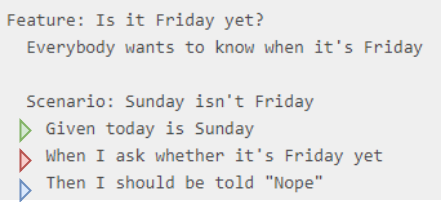
\includegraphics[width=\textwidth]{images/dslReturn.png}
                \caption{Retour des tests au niveau des exigences}
                \label{ref:colors}
            \end{figure}
            
Si le test n'a pas été trouvé, rien n'est affiché près du mot clé. Ainsi, toutes les parties prenantes ont une vision claire des exigences et peuvent en un lancement de test déterminer quelles exigences ont été respectées ou non.

\section{Critique de la solution}

Nous avons tenté de proposer une solution aux lacunes que d'autres outils possédaient. Toutefois, nous pensons que nous devons travailler sur quelques points pour l'améliorer.

Dans la solution proposée, les développeurs doivent manuellement effacer un commentaire de type \textit{TODO} dès qu'ils terminent d'implanter la méthode pour signifier que la méthode n'est plus à implanter. Leur donner le droit d'effacer un commentaire c'est aussi leur donner le droit d'en écrire. Un développeur peut écrire des assertions basiques pour tester une méthode. Par exemple, si un développement implante toutes les méthodes en écrivant :
\begin{lstlisting}
@Given("^today is Sunday$")
public void today_is_Sunday(){
assert.equals("Test","Test")
throw new PendingException();
}
\end{lstlisting}

Dans ce cas là toutes les méthodes retourneront un résultat OK à chaque lancement des tests. Donc toutes les notations graphiques seront au vert, ce qui fausse la réalité. Nous avons donc pas de moyen de vérifier la qualité de l'implantation du test. 

